  \mysection{The Philosopher}{trope-philosopher}

  \flavor{Holy Diver!  You've been down too long in the midnight sea ... \Tilde Dio, "Holy Diver"}


  \mysubsection{The Basics}{philosopher-basics}


  \myhighlight{Supple}{philosopher-flesh}

  Philosophers have a d6 \FLESH


  \myhighlight{Genius}{philosopher-genius}

  Philosophers add their \LVL to any \RO or \RB attempt they're trying that includes their \INT 

  

  \mysubsection{Creation}{philosopher-creation}

  \callout{
    \mynumlist {
      \item Move any of your core Skills \DCUP
      \item Move any of your core Saves \DCUP
      \item Pick \mybold{three} \mylink{Virtues}{philosopher-virtues} from the list below.  You can only pick each Virtue once.
      \item Pick \mybold{one} \mylink{Complication}{philosopher-complications} from the list below (or make up your own with the Arbiter!)
      \item Write down your Starting Gear
    }
  }

  \begin{center}
  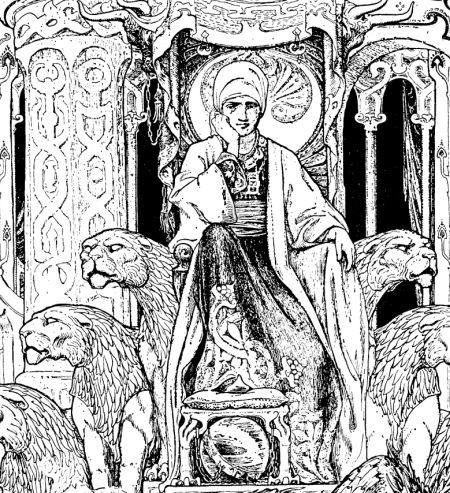
\includegraphics[scale=.5]{Philosopher}
  \end{center}

    \mytable{X}{
      \thead{\mysubsection{Virtues}{philosopher-virtues}} \\
    }{
      \mylink{College}{philosopher-virtue-college} \\
      \mylink{The Crux of Blood}{philosopher-virtue-blood} \\
      \mylink{The Crux of Knowledge}{philosopher-virtue-knowledge} \\
      \mylink{Intangibles}{philosopher-virtue-intangibles} \\
      \mylink{Invocation}{philosopher-virtue-invocation} \\
      \mylink{Leechcraft}{philosopher-virtue-leechcraft}  \\
      \mylink{Research: Chymistry}{philosopher-virtue-research} \\
      \mylink{Research: Inscription}{philosopher-virtue-research}  \\
      \mylink{Research: Medicinals}{philosopher-virtue-research}  \\
      \mylink{Wonder: Staff Magic}{philosopher-virtue-staff-magic} \\
    }

  \newpage

    \myhighlight{College}{philosopher-virtue-college}

    \flavor{Christ. Seven years of college down the drain. \Tilde "Bluto" Blutarsky, Animal House}

    You received an education and some equipment from one of the many Philosopher's Colleges that dot the major cities of Acheron.  You start with \mybold{three} of the following:


    \dashedbox {
      \mybullet {
      \item a Polearm;
      \item a Grimoire with 5 spells of your choice (these spells can be added to a Grimoire if you already have one);
      \item a set of two silver daggers;
      \item a Fetish with d4 \UD of any spell you choose;
      \item a suit of Light or Medium armor (incompatible with Wizardry);
      \item 5 picks from the \mylink{Adventuring Gear}{gear-adventuring} table;
      \item a pouch of 3 gems (roll on the \mylink{Gems table}{appendixb-random-treasure} in Appendix B);
      \item d4 \UD of a Narcotic of your choice;
      \item a Staff or Caduceus with 1 Iron ability (see \mylink{Staff Magic}{wonder-staff-magic})
    }}

  \myhighlight{The Crux of Blood}{philosopher-virtue-blood}

  \flavor{You push yourself to the edge of madness and reason, riding the warp and weft of the fabric of existence to master the arcane words that are gibbered and shrieked by the creatures beyond the Void.  They seek blood in payment - the sap of  Ygg, the brine of the Six Seas, the fire inside the calderas that felled Atlantis.  Blood is Life, and they desire it more than anything.  Blood aids great sorcery. Blood is Power.}

  When you learn the Crux of Blood, choose a \mylink{Wizardry spell}{arcana-wizardry}.  This spell is etched on the inside of your cranium "...like moth larvae burrowing through the bark of a tree."  This spell can be cast without speaking or moving.  If someone cuts off your head and scoops out your brains, they can read (and learn) the spell too (see \mylink{Fetishes}{philosopher-fetishes}).

  Learning this Virtue also permits you to harvest \mylink{Components}{philosopher-components} from fallen foes in order to make casting your arcana more effective.

  The Crux of Blood grants you a single d6 \POOL die - the Blood Die - that you can use to perform \mylink{Wizardry}{arcana-wizardry}.  This Blood Die is in addition to the one you would receive from \mylink{Invocation}{philosopher-virtue-invocation}, should choose that Virtue.


  \myhighlight{The Crux of Knowledge}{philosopher-virtue-knowledge}

  \flavor{Magic exists.  Undeniably.  But those who try to control \myital{arcana} are buffeted by it, controlled by it, consumed by it.  Slain by it.  Science, however, is \myital{our} creation.  It exists to serve - humble, obedient, and aloof.  Few have the discipline to seduce it; it takes a lifetime of dedication, a lifetime of asking "why?" over and over again and knowing that there will be no end to the question.  "Why?" will reverberate in the heavens when the last star winks out.  "Why?" is a quest, a calling.  It drives us to travel the heights and depths, tame the riches of the world, cheat death and defy Chance and spit in the face of Luck.  When you walk the path of "Why?", you follow in the footsteps of Gods.}


  You gain 1 d10 Knowledge \STATIC.  You use this Knowledge Die to practice the Arcana of \mylink{Leechcraft}{arcana-leechcraft}. Choose a single \mylink{Remedy}{arcana-leechcraft} you know how to perform (and no other).

  The Crux of Knowledge also bestows an honorific on the practitioner; your title will be used in "polite society".   


    \mytable{X r}{
      \thead{Honorific} & \thead{Knowledge Die} \\
    }{
      Honorable & d10 \STATIC \\
      Professor & d12 \STATIC \\
      Doctor & d16 \STATIC \\
      Maestro & d20 \STATIC \\
    }

   

  The \STATIC Knowledge from the Crux of Knowledge \mybold{replaces} the one you gain from \mylink{Leechcraft}{philosopher-virtue-leechcraft}, should choose that Virtue 


  \myhighlight{Intangibles}{philosopher-virtue-intangibles}

    You may move two different Intangible Stats of your choice \DCUP.  Describe to the Arbiter why these Intangible Stats are better than average.

 
  \myhighlight{Invocation}{philosopher-virtue-invocation}

   \flavor{\myital{Klaatu barada nikto!} \\~ \Tilde "The Day the Earth Stood Still" / "Army of Darkness"}

   You take possession of a \mylink{Grimoire}{philosopher-grimoires} with 3 \mylink{Wizardry}{arcana-wizardry} arcana inscribed in it.  The arcana must be \mylink{chosen randomly}{table-random-spells}.  The Grimoire has your \mylink{Wizard Sigil}{research-sigil-wizard} inscribed on it, and is trapped.
  
  Invocation grants you a single d6 \POOL die - the Blood Die - that you can use to perform \mylink{Wizardry}{arcana-wizardry}.  This Blood Die is in addition to the one you would receive from \mylink{the Crux of Blood}{philosopher-virtue-blood}, should you choose that Virtue.


  \myhighlight{Leechcraft}{philosopher-virtue-leechcraft}

  \flavor{"I suppose nothing hurts you."  "... Only pain" \\~ \Tilde Conan the Destroyer}
  
   You gain 1 d6 Knowledge \STATIC.  Use this Knowledge Die to practice \mylink{Leechcraft}{arcana-leechcraft}.  You know how to perform \mybold{all} the \mylink{Remedies}{arcana-leechcraft} listed under Leechcraft.

   If you have the Virtue \mylink{Crux of Knowledge}{philosopher-virtue-knowledge}, this d6 Knowledge \STATIC is \mybold{replaced by} the one you gain from that Virtue.



 \myhighlight{Research}{philosopher-virtue-research}

  \flavor{I collect molds, spores, and fungus.  \\~ \Tilde Egon Spengler, "Ghostbusters"}
  
  There are 3 major types of Research : Chymistry, Medicinals, and Inscription.  For each type of Research you learn, you gain 1 point of Research.

  You use your Research during a Vacation.  Your Research doesn't "roll over" between Vacations, and resets itself at the start of each Vacation.

  \cbreak

  \dashedbox {



  \myital{\hypertarget{philosopher-virtue-chymistry}{Chymistry}}

   Create potions and salves, toxins and acids. Gain 1 point of Research \\~

  \myital{\hypertarget{philosopher-virtue-inscription}{Inscription}}
  
   Read and write magical texts and inscriptions. Gain 1 point of Research \\~

  \myital{\hypertarget{philosopher-virtue-medicinals}{Medicinals}}

  Cure diseases, addictions, wounds, and madness through the power of science. Gain 1 point of Research \\~

}%end dashed box

 \myhighlight{Wonder: Staff Magic}{philosopher-virtue-staff-magic}

  \flavor{His staff! I told you to take the Wizard's staff! \\~ \Tilde Grima Wormtongue, The Two Towers}  

  Create a \mylink{Magic Staff or Caduceus}{wonder-staff-magic}



  \begin{center}
  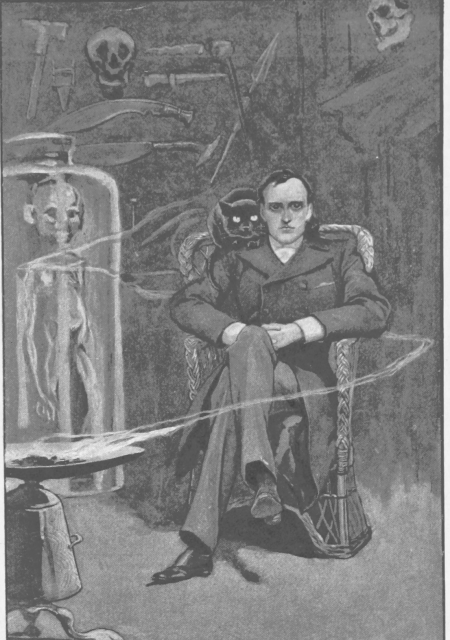
\includegraphics[scale=.45]{Philosopher_2}
  \end{center}


    \mytable{X}{
      \thead{\mysubsection{Complications}{philosopher-complications}} \\
    }{
      Bibliophile \\
      It is I - Balthazar the Breathtaking! \\
      Logical \\
      Morbid \\
      Mysophobia \\
      Necronomicon \\
      One More Page \\
      Out of Shape \\
      Whoops! \\
      Transcendental Research \\
    }


  \myhighlight{Bibliophile}{philosopher-bibliophile}          

  You really, really love books. If given the choice between a share of treasure and a book you haven't read, you will opt for the book every time.  You will look to build a library and hire porters to carry spare books around for you.  The books you covet must be unusual or educational (practically, this means grimoires or books that teach or augment Skills).  You must have at least 3 Significant Items worth of books with you at all times.  Tell the Arbiter about your favorite book.

  \myhighlight{It is I - Balthazar the Breathtaking!}{philosopher-complication-arrogance}

  There's your typical run-of-the-mill arrogance - braggarts, blowhards, and boasters - and then there's you.  Your arrogance is on a whole other level.  You won't tolerate any other Philosophers in your Band.  You accept no masters and believe in no law but your own. To "the Man", you are an appalling spectacle, and should be put in your place (or in the ground) before you harm anyone else.

  \myhighlight{Logical}{philosopher-logical}

  You are devoid of any emotion.  People call you cold, distant, or calculating.  When faced with a decision or dilemma, you will always opt for the logical, unemotional solution.

  \myhighlight{Morbid}{philosopher-morbid}

  You require corpses - the fresher, the better - to perform Research (Chymistry, Inscription, or Medicinals).  You'll need at least 1 fresh corpse if you want to use Research during a \mylink{Vacation}{civilization-vacation}. 

  \myhighlight{Mysophobia}{philosopher-mysophobia}

  You have an morbid fear of "contamination".  You wear a mask and gloves that you rarely take off, insist on cleanliness whenever possible, keep your clothing and gear in neat order, and bathe often. Tell the Arbiter how you got this way.

  \myhighlight{Necronomicon}{philosopher-necronomicon}

  You are in possession of a forbidden tome, text, or fetish.  It's taught you everything you need to know and (quite possibly) made you slightly insane.  All of your Research (Chymistry, Inscription, or Medicinals) has to start with this book; practically, you have to \RS: Sanity whenever you spend any Research.  Tell the Arbiter what this book is, and how you got it.

  \myhighlight{One More Page}{philosopher-one-more-page}

  During a Bivouac, you can't seem to stop reading, writing, drawing, or hypothesizing.  You must make a \RS: \FOC check when you take a Bivouac, in addition to your Provision roll.  If you Fail (roll a 1 or a 2), you don't get any of the benefits of having rested.

 \myhighlight{Out of Shape}{philosopher-out-of-shape}

  You're a little (OK, a lot) out of shape.  One of your Significant Item slots is taken up by your excess weight, and you aren't able to run for longer than Minutes.

  \myhighlight{Transcendental Research}{philosopher-transcendental-research}

  You require narcotics to do Research (Chymistry, Inscription, or Medicinals).  Pick a \mylink{Narcotic}{gear-narcotics}; you must roll a \UD of this Narcotic any time you spend Research during a \mylink{Vacation}{civilization-vacation}.

  \myhighlight{Whoops!}{philosopher-whoops}

  An experiment or spell went awry some time in your past.  Roll twice on the \mylink{Mishaps table}{table-mishap}

  \mysubsection{Starting Gear}{philosopher-starting-gear}


\mybullet {
    \item a bedroll; 
    \item a book hanger;
    \item a pipe and d4 \UD of tobacco;
    \item a quarterstaff;
    \item one pick OR 3 rolls on the \mylink{Random Items}{appendixb-random-items} table in Appendix B;
  }

\newpage


\mysubsection{Examples}{philosopher-examples}

\myhighlight{The Doctor}{philosopher-doctor}

\example{Lore, Crux of Knowledge, Leechcraft, Research:Medicinals, Morbid}

\myhighlight{The Sorcerer}{philosopher-sorcerer}

\example{Lore, Crux of Blood, Wizardry, Research:Inscription, Whoops!}

\myhighlight{The Alchemist}{philosopher-alchemist}

\example{Eyeball, Research: Inscription, Research: Chymistry, College, Transcendental Research}

\newpage
